%    MetaUML: Tutorial, Reference and Test Suite
%
%    Copyright (c) 2005-2019 Ovidiu Gheorghies
%    Permission is granted to copy, distribute and/or modify this document
%    under the terms of the GNU Free Documentation License, Version 1.2
%    or any later version published by the Free Software Foundation;
%    with no Invariant Sections, no Front-Cover Texts, and no Back-Cover Texts.
%    A copy of the license is included in the section entitled "GNU
%    Free Documentation License".

\documentclass{article}

\usepackage[utf8]{inputenc}
\usepackage[pdftex,colorlinks=true]{hyperref}
\usepackage{multicol}
\usepackage{multido}
\usepackage[style=ieee]{biblatex}
\addbibresource{metauml-manual.bib}

\ifx\pdftexversion\undefined
  \usepackage[dvips]{graphicx}
\else
  \usepackage[pdftex]{graphicx}
   \DeclareGraphicsRule{*}{mps}{*}{}
\fi

\newcommand{\code}{\ttfamily}

\setcounter{page}{1}

\begin{document}

MetaUML: A Manual and Test Suite

\begin{quote}
    Copyright \copyright 2005-2019 Ovidiu Gheorghie\c{s}.
    Permission is granted to copy, distribute and/or modify this document
    under the terms of the GNU Free Documentation License, Version 1.2
    or any later version published by the Free Software Foundation;
    with no Invariant Sections, no Front-Cover Texts, and no Back-Cover Texts.
\end{quote}

\pagebreak
This page is intentionally left blank.

\pagebreak
\title{MetaUML: A Manual and Test Suite}

\author{Ovidiu Gheorghie\c{s}}

\maketitle

\begin{abstract}
MetaUML is a MetaPost \cite {metapost} library for creating UML \cite{umlomg} diagrams by means of a textual notation.
While presenting the inner workings of MetaUML, this manual doubles as a step-by-step tutorial.
More importantly, its source code contains many useful examples of diagrams, ranging from the very basic to the
more advanced and customized.
\end{abstract}

\section{Introduction}

Here is a quick MetaUML showcase:

\begin{multicols}{2}
\paragraph{A} Class Diagram\\
\includegraphics[scale=.55]{fig/appetizer.1}
\paragraph{B} Activity Diagram\\
\includegraphics[scale=.55]{fig/appetizer.2}
\paragraph{C} Notes\\
\includegraphics[scale=.55]{fig/appetizer.5}
\columnbreak
\paragraph{D} Use Case Diagram\\
\includegraphics[scale=.55]{fig/appetizer.3}
\paragraph{E} State Machine Diagram\\
\includegraphics[scale=.55]{fig/appetizer.4}
\paragraph{F} Package Diagram\\
\includegraphics[scale=.55]{fig/appetizer.6}
\end{multicols}

\pagebreak

The code that generates these diagrams is quite straightforward, combining a natural object-oriented parlance
with the power of MetaPost equation solving.

For example, a UML class is drawn as follows:

\begin{multicols}{2}
\begin{verbatim}
Class.A("MyClass")
  ("attr1: int", "attr2: int")
  ("method1(): void",
   "method2(): void");

A.nw = (0, 0); % optional, implied
drawObject(A);
\end{verbatim}
\columnbreak
\hspace{1cm}\includegraphics{fig/appetizer.7}
\end{multicols}

This code creates a visual object, referenced by its name {\code A}, of the MetaUML-defined type {\code Class}. 
Object {\code A} has the following content properties: a name
({\code MyClass}), a list of attributes ({\code attr1}, {\code attr2})
and a list of methods ({\code method1}, {\code method2}). To set the object's location, we assign a value to the 
so-called ``north-west'' point of the encompassing rectangle, {\code A.nw} --- a point which in actual fact references 
the upper-left corner.

Every MetaUML visual object has the layout properties shown in figure \ref{fig:properties}. 
These properties may be used to set the location of any given object, either by assigning to them absolute values,
or by linking them relatively to other objects via equations.

\begin{figure}
\centering
\includegraphics{fig/properties.1}
\caption{Layout properties of MetaUML objects. Here, a {\code Class} object is depicted.}
\label{fig:properties}
\end{figure}
 
The following example demonstrates, respectively, the use of absolute and relative positioning for two classes, {\code A} and {\code  B}.

\begin{multicols}{2}
\begin{verbatim}
A.nw = (0,0);
B.w = A.e + (20, 0);
\end{verbatim}
\columnbreak
\includegraphics{fig/appetizer.8}
\end{multicols}

After the objects have been drawn, it becomes possible to attach links to them. In a class diagram, inheritance
or association relations are meaningful links between classes, while in a state machine diagram, transitions between 
states can be used. Here is the general pattern used by MetaUML for drawing links:

\begin{verbatim}
link(<how-to-draw-information>)(<path-to-draw>);
\end{verbatim}

The ``how-to-draw-information'' is an object which defines the style of the line (e.g. solid, dashed) and the appearance
of the heads (e.g. nothing, arrow, diamond). One such object, appropriately called {\code inheritance}, defines a solid
line style and a white triangle head. The other parameter, the ``path-to-draw'', is simply a MetaPost path.

For example, the following call draws an inheritance relation from class {\code B} to class {\code A}.

\begin{verbatim}
link(inheritance)(B.e -- A.w);
\end{verbatim}

The direction of the path is important, as MetaUML uses it to determine the
type of adornment to attach to the link ends (if applicable). In our example, a white triangle,
denoting inheritance, points towards the end of the path, that is towards class {\code A}.

Let us sum up with a diagram typical for MetaUML use. Firstly, we define the objects that we want to include
in our diagram. Secondly, we position these objects relative to each other. Thirdly, we draw the objects. Finally, we
draw the links, by referencing the layout properties of the previously drawn objects. Note that in our example the
positioning of {\code A} need not be set explicitly because ``floating'' objects are automatically positioned at 
{\code (0,0)} by their draw method.

\begin{multicols}{2}

\begin{verbatim}
input metauml;

beginfig(1);
  Class.A("A")()();              % 1. Define the objects
  Class.B("B")()();
  B.w = A.e + (20, 0);           % 2. Position the objects
  drawObjects(A, B);             % 3. Draw the objects
  link(inheritance)(B.w -- A.e); % 4. Draw links between objects
endfig;
end
\end{verbatim}
\columnbreak
\includegraphics{fig/appetizer.9}
\end{multicols}

As far as a user is concerned, this is all there is to MetaUML. With a reference describing how the
UML elements are created, arbitrarily complex diagrams can be crafted.

\section{Class Diagrams}

A class is created as follows:

\begin{verbatim}
Class.<name>(<class-name>)
  (<list-of-attributes>)
  (<list-of-methods>);
\end{verbatim}

The suffix {\code <name>} specifies an identifier for the newly created {\code Class} object 
(which, of course, represents a UML class).
The name of the UML class is a string given by {\code <class-name>};
the attributes and methods are given as list of strings, {\code <list-of-attributes>} and {\code <list-of-methods>} 
respectively. The list of attributes and the list of methods may be void.

An attribute or a method string may begin with a visibility marker: ``$+$'' for
public, ``\#'' for protected, ``$-$'' for private, and ``\textasciitilde'' for package private. 
The default visibility is package private.

\begin{multicols}{2}
\begin{verbatim}
Class.A("Point")
  ("#x:int", "#y:int")
  ("+set(x:int, y:int)",
   "+getX():int",
   "+getY():int",
   "-debug():void",
   "test():void");
drawObject(A);
\end{verbatim}
\columnbreak
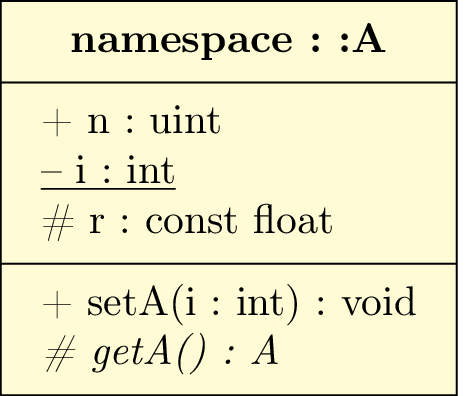
\includegraphics{fig/class.1}
\end{multicols}

To disable showing the visibility markers, use {\code Class\_noVisibilityMarkers}, as shown below:

\begin{multicols}{2}
\begin{verbatim}
  Class.A("Point")
    ("#x:int", "#y:int")
    ("+toString():String");
  Class_noVisibilityMarkers.A;

  drawObject(A);
\end{verbatim}
\columnbreak
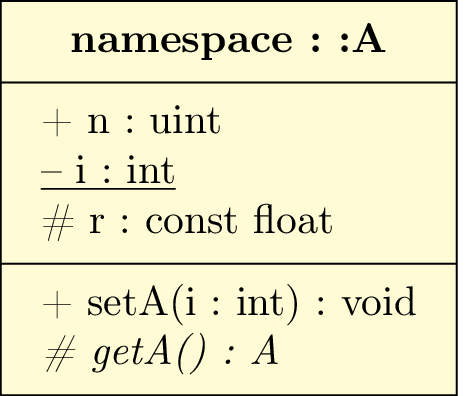
\includegraphics{fig/class.15}
\end{multicols}

\subsection{Stereotypes}

After a class is created, but before it is drawn, its stereotypes may be specified by using {\code Class\_stereotypes}:

\begin{verbatim}
Class_stereotypes.<name>(<list-of-stereotypes>);
\end{verbatim}

Here, {\code <name>} is the object name of a previously created class and {\code <list-of-stereotypes>}
is a comma-separated list of strings. Here is an example:

\begin{multicols}{2}
\begin{verbatim}
Class.A("User")()();
Class_stereotypes.A("<<interface>>","<<home>>");

drawObject(A);
\end{verbatim}
\columnbreak
\hspace{3cm}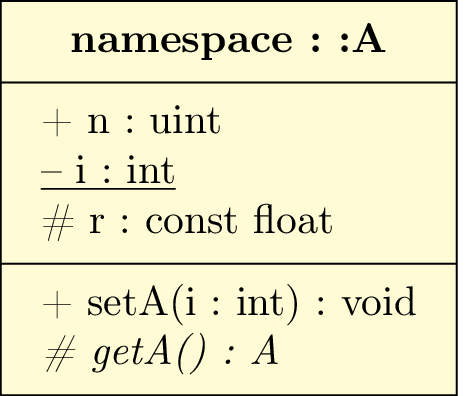
\includegraphics{fig/class.2}
\end{multicols}

\subsection{Interfaces and Abstract Classes}

At times it is preferred to write the name of an interface in an oblique font, rather than using the ``interface''
stereotype. This can be easily achieved by using the macro {\code Interface}:

\begin{verbatim}
Interface.name(class-name)
  (list-of-methods);
\end{verbatim}

Here is an example:

\begin{multicols}{2}
\begin{verbatim}
Interface.A("Observer")
    ("+update(src:Object)");

drawObject(A);
\end{verbatim}
\columnbreak
\hspace{1cm}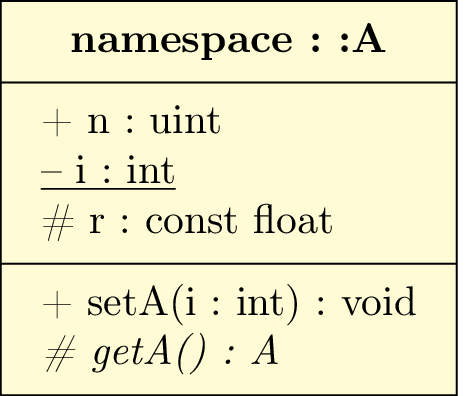
\includegraphics{fig/class.11}
\end{multicols}

Since internally {\code Interface} treated as a special kind of {\code Class}, the code above is equivalent to:
\begin{verbatim}
EClass.A(iInterface)("Observer")()
      ("+update(src:Object)");
\end{verbatim}

Abstract classes can be drawn similarly using the {\code iAbstractClass} style:
\begin{samepage}
\begin{multicols}{2}
\begin{verbatim}
EClass.A(iAbstractClass)("Observable")
    ("observers: Observer[0..*]")
    ("+addObserver(o: Observer)",
     "+notify()");

drawObject(A);
\end{verbatim}
\columnbreak
\hspace{1cm}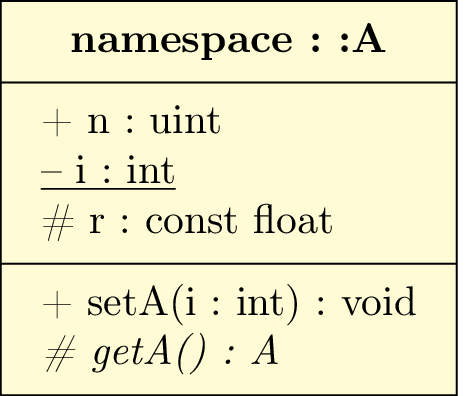
\includegraphics{fig/class.12}
\end{multicols}
\end{samepage}

If you prefer, you can use equivalent construct:

\begin{verbatim}
AbstractClass.A("Observable")
    ("observers: Observer[0..*]")
    ("+addObserver(o: Observer)",
     "+notify()");
\end{verbatim}

\subsection{Displaying Class Name Only}

If you want the empty methods and attributes compartments in a class not being displayed, one way is to set the spacing
at their top and the bottom to {\code 0}:
\begin{samepage}
\begin{multicols}{2}
\begin{verbatim}
Class.A("MyModel")()();
A.info.iName.top    := 10;
A.info.iName.bottom := 10;
A.info.iAttributeStack.top := 0;
A.info.iAttributeStack.bottom := 0;
A.info.iMethodStack.top := 0;
A.info.iMethodStack.bottom := 0;

drawObject(A);
\end{verbatim}
\columnbreak
\hspace{1cm}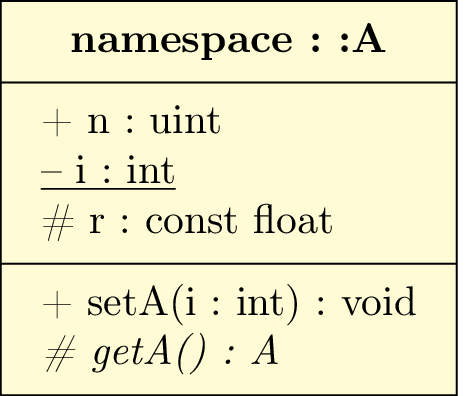
\includegraphics{fig/class.13}
\end{multicols}
\end{samepage}

The same effect can be achieved by using the formatting information object {\code iClassNameOnly} or the {\code ClassName} macro:

\begin{multicols}{2}
\begin{verbatim}
EClass.A(iClassNameOnly)("MyModel")()();
ClassName.B("AnotherModel");
Class_stereotypes.B("<<smart>>");

topToBottom(20)(A, B);

drawObjects(A, B);
\end{verbatim}
\columnbreak
\hspace{2cm}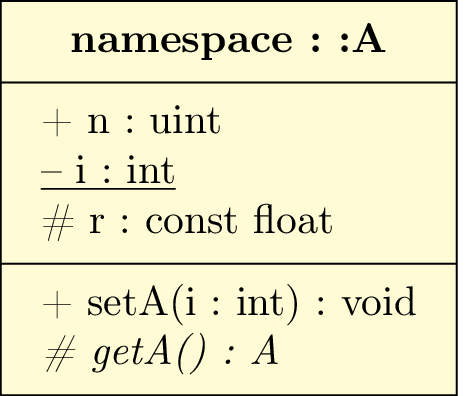
\includegraphics{fig/class.14}
\end{multicols}

To customize the space around the class name globally, you can set the values of {\code iClassNameOnly.iName.top} and {\code iClassNameOnly.iName.bottom}. Individually, for a given object, say {\code B}, the attributes {\code B.info.iName.top} and {\code B.info.iName.bottom} can be used.

\subsection{Objects (or Class Instances)}

A UML object (or class instance) is created as follows:

\begin{verbatim}
Instance.name(object-name)
  (list-of-attributes);
\end{verbatim}

The suffix {\code name} gives a name to the {\code Instance} object. The name of the object (given by {\code object-name}) is typeset underlined. The attributes are given as a comma-separated list of strings, {\code list-of-attributes}.

\begin{multicols}{2}
\begin{verbatim}
Instance.order("o: Order")
  ("name='book'", "{placed}", "{payed}");
drawObject(order);
\end{verbatim}
\columnbreak
\hspace{2cm}\includegraphics{fig/instance.1}
\end{multicols}


\subsection{Parametrized Classes (Templates)}

The most convenient way of typesetting a class template in MetaUML is to use the macro {\code ClassTemplate}.
This macro creates a visual object which is appropriately positioned near the class object it adorns.

\begin{verbatim}
ClassTemplate.name(list-of-templates)
                  (class-object);
\end{verbatim}

The {\code name} is the name of the template object, {\code list-of-templates} is a comma-separated list of strings and the {\code class-object} is the name of a class object.

Here is an example:

\begin{multicols}{2}
\begin{verbatim}
Class.A("Vector")()();
ClassTemplate.T("T", "size: int")(A);

drawObjects(A, T);
\end{verbatim}
\columnbreak
\hspace{1cm}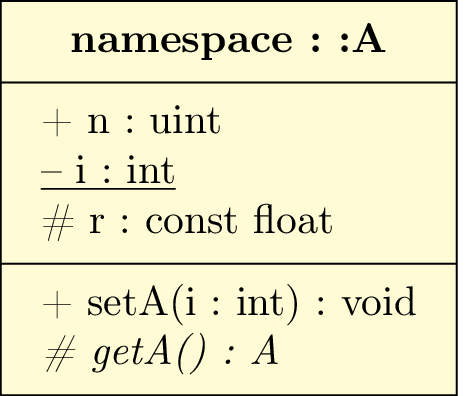
\includegraphics{fig/class.3}
\end{multicols}

The macro {\code Template} can also be used to create a template object, but this time the resulting
object can be positioned freely.

\begin{verbatim}
Template.name(list-of-templates);
\end{verbatim}

Of course, it is possible to specify both stereotypes and template parameters for a given class.

\subsection{Types of Links}

In this section we enumerate the relations that can be drawn between classes by means
of MetaUML macros. Suppose that we have the declared two points, {\code A} (on the left)
and {\code B} (on the right):

\begin{verbatim}
pair A, B;
A = (0,0);
B = (50,0);
\end{verbatim}

\begin{tabular}{||l|c||}
\hline
{\code link(association)(X.e -- Y.w)} & \includegraphics{fig/class_diagrams.4} \\
\hline
{\code link(associationUni)(X.e -- Y.w)} & \includegraphics{fig/class_diagrams.5}  \\
\hline
{\code link(inheritance)(X.e -- Y.w)} & \includegraphics{fig/class_diagrams.6} \\
\hline
{\code link(realization)(X.e -- Y.w)} & \includegraphics{fig/class_diagrams.12} \\
\hline
{\code link(aggregation)(X.e -- Y.w)} & \includegraphics{fig/class_diagrams.7} \\
\hline
{\code link(aggregationUni)(X.e -- Y.w)} & \includegraphics{fig/class_diagrams.8} \\
\hline
{\code link(composition)(X.e -- Y.w)} & \includegraphics{fig/class_diagrams.9} \\
\hline
{\code link(compositionUni)(X.e -- Y.w)} & \includegraphics{fig/class_diagrams.10} \\
\hline
{\code link(dependency)(X.e -- Y.w)} & \includegraphics{fig/class_diagrams.11} \\
\hline
\end{tabular}

\subsection{Associations}
In UML an association typically has two of association ends and may have a name specified for it.
In turn, each association end may specify a multiplicity, a role, a visibility, an ordering.
These entities are treated in MetaUML as pictures having specific drawing information
(spacings, font).

The first method of creating association ``items'' is by giving them explicit names.
Having a name for an association item comes in handy when referring to its properties
is later needed (see the non UML-compliant diagram below). The last parameter of the macro {\code item} is an equation which may use the item's name to perform positioning.

\begin{multicols}{2}
\begin{verbatim}
Class.P("Person")()();
Class.C("Company")()();
% drawing code ommited

item.aName(iAssoc)("works for")
          (aName.s = .5[P.w, C.w]);
draw aName.n -- (aName.n + (20,20));
label.urt("association name" infont "tyxtt",
          aName.n + (20,20));
\end{verbatim}
\columnbreak
\hspace{1cm}\includegraphics[scale=.8]{fig/class_association.1}
\end{multicols}

However, giving names to every association item may become an annoying burden
(especially when there are many of them). Because of this, MetaUML also allows for
``anonymous items''. In this case, the positioning is set by an equation
which refers to the anonymous item as {\code obj}.

\begin{multicols}{2}
\begin{verbatim}
% P and C defined as in the previous example

item(iAssoc)("employee")(obj.nw = P.s);
item(iAssoc)("1..*")(obj.ne = P.s);

% other items are drawn similarly
\end{verbatim}
\columnbreak
\hspace{3cm}\includegraphics{fig/class_association.2}
\end{multicols}

\subsection{Dependencies and Stereotypes}

Stereotypes are frequently used with dependencies. Below is an example.
\pagebreak

\begin{multicols}{2}
\begin{verbatim}
Class.F("Factory")()();
Class.O("Object")()();

O.n = F.s - (0, 50);
drawObjects(F, O);

clink(dependency)(F, O);
item(iStereo)("<<creates>>")(obj.w = .5[F.s,O.n])
\end{verbatim}
\columnbreak
\hspace{3cm}\includegraphics{fig/class_association.3}
\end{multicols}

\section{Notes}

A note is created as follows:

\begin{verbatim}
Note.name(list-of-lines);
\end{verbatim}

The suffix {\code name} is the name of the {\code Note} object. The contents of the note is given by a comma-separated
list of strings, {\code list-of-lines}, gives the text contents of the note object, each string being drawn on its own
line.

Here is an example:

\begin{multicols}{2}
\begin{verbatim}
Note.A("This note", "has two lines.");
drawObject(A);
\end{verbatim}
\columnbreak
\hspace{3cm}\includegraphics{fig/note.1}
\end{multicols}

\subsection{Attaching notes to diagram elements}

Notes can be attached to diagram elements by using a link of type {\code dashedLink}.

\begin{multicols}{2}
\begin{verbatim}
Note.A("This is a class");
Class.C("Object")()();

A.sw = C.ne + (20, 20);

drawObject(A, C);

clink(dashedLink)(A, C);
\end{verbatim}
\columnbreak
\hspace{1cm}\includegraphics{fig/note.2}
\end{multicols}

Now let us see a more complex example, which demontrates the ability of accessing sub-elements in a MetaUML diagram.
\pagebreak

\begin{multicols}{2}
\begin{verbatim}
Note.nA("This is the class name");
Note.nB("This is a key attribute");
Note.nC("This is a nice method");

Class.C("Object")("+id:int")
        ("+clone()", "+serialize()");

topToBottom.left(10)(nA, nB, nC);
leftToRight(10)(C, nB);

drawObjects(C, nA, nB, nC);

clink(dashedLink)(C.namePict, nA); 
clink(dashedLink)(C.attributeStack.pict[0], nB); 
clink(dashedLink)(C.methodStack.pict[1], nC);
\end{verbatim}
\columnbreak
\hspace{1cm}\includegraphics{fig/note.3}
\end{multicols}

Macros like {\code leftToRight} and {\code topToBottom} are presented in section \ref{section:positioning}.

\subsection{Using mathematical formulae}

MetaUML notes can contain mathematical formulae written in TeX \cite{texbook}. Regretably, LaTeX \cite{latexbook} support for formulae is {\bf not} available.
Limited as it may be, this feature is considered experimental, as it is not always straightforward to use. In the example below, note that the MetaPost package {\code TEX} is imported.

\begin{multicols}{2}
\begin{verbatim}
input metauml;
input TEX;

beginfig(1);
    Note.A("This class implements the formula:", 
           TEX("$\sum_1^n f(x) \cdot dx$"));
    drawObjects(A);
endfig;

end
\end{verbatim}
\columnbreak
\hspace{0.5cm}\includegraphics{fig/note.4}
\end{multicols}

For taller formulae, you must be prepared to do some advanced stunts. Remark: {\code "aaa" \& "bbb"} is MetaPost's way to concatenate the strings into {\code "aaabbb"};
the string containing the formula was split in two for layout reasons.

\begin{multicols}{2}
\begin{verbatim}
Note.A("Can you do it?", 
        TEX("$\sum_1^n f(x) \cdot dx " &
            "\over \sum_1^m g(y) \cdot dy$"));
A.stack.info.spacing := 30;
A.stack.pict[1].info.ignoreNegativeBase := 0;

drawObject(A);
\end{verbatim}
\columnbreak
\hspace{3cm}\includegraphics{fig/note.5}
\end{multicols}

Alas, this trick does not entirely solve the problem: a third line in the note would be badly aligned. Therefore,
until MetaUML's {\code Note} class is upgraded to better support this scenario, you may want to limit yourself 
to two lines per note --- at least when tall formulae are involved.

\section{Packages}

MetaUML allows for the creation of packages in various forms. Firstly, we have the option of writing the package 
name in the middle of the main box. Secondly, we can write the name on the tiny box above the main box, leaving 
the main box empty. Lastly, we can write the package name as in the second case, but the main box can have an arbitrary
contents: classes, other packages, or even other UML items. 

The macro that creates a package has the following synopsis:

\begin{verbatim}
Package.name(package-name)(subitems-list);
\end{verbatim}

The parameter {\code package-name} is a string or a list of comma-separated strings representing the package's name.
The {\code subitems-list} parameter is used to specify the subitems (tipically classes or packages) of this package;
its form is as a comma-separated list of objects, which can be void.

\begin{multicols}{2}
\begin{verbatim}
Package.P("java.lang")();
drawObject(P);
\end{verbatim}
\columnbreak
\hspace{3cm}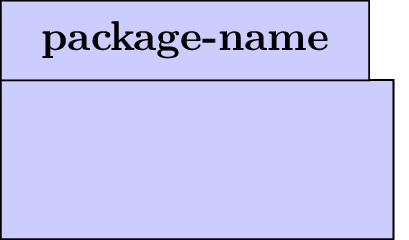
\includegraphics{fig/package.1}
\end{multicols}

Below is another example:

\begin{multicols}{2}
\begin{verbatim}
Package.P("An important", "package")();
drawObject(P);
\end{verbatim}
\columnbreak
\hspace{3cm}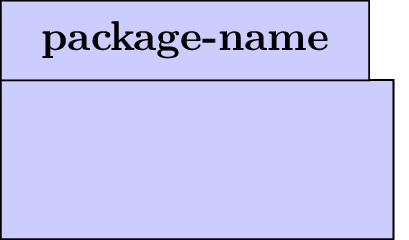
\includegraphics{fig/package.2}
\end{multicols}

If you wish to leave the main box empty, you can use the following code:

\begin{multicols}{2}
\begin{verbatim}
Package.P("java.lang")();
P.info.forceEmptyContent := 1;
drawObject(P);
\end{verbatim}
\columnbreak
\hspace{3cm}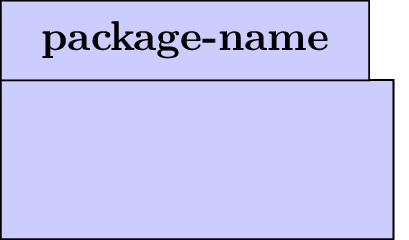
\includegraphics{fig/package.3}
\end{multicols}

The same effect as above can be achieved globally by doing:

\begin{verbatim}
iPackage.forceEmptyContent := 1;
\end{verbatim}

More information on MetaUML's way of managing global and per-object configuration data can be found in
section \ref{section:infrastructure} and section \ref{section:customization}.

Here is an example involving items contained in a package.

\begin{multicols}{2}
\begin{verbatim}
Class.A("A")()();
Class.B("B")()();
Package.P("net.metauml")(A, B);

leftToRight(10)(A, B);

drawObject(P);
\end{verbatim}
\columnbreak
\hspace{3cm}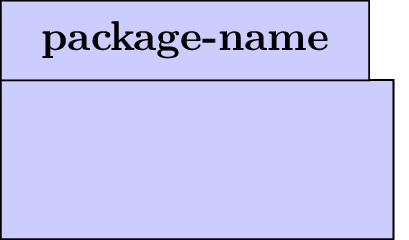
\includegraphics{fig/package.4}
\end{multicols}

\subsection{Types of Links}

The nesting relation between packages is created by using the {\code nest} link information.

\begin{tabular}{||l|c||}
\hline
{\code link(nest)(X.e -- Y.w)} & 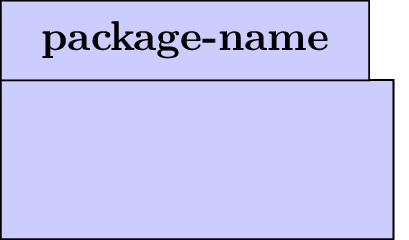
\includegraphics{fig/package.5} \\
\hline
\end{tabular}

\section{Component Diagrams}

A component is created by the macro {\code Component}:

\begin{verbatim}
Component.name(component-name)
  (subitems-list)
\end{verbatim}

The parameter {\code component-name} is a string representing the component's name. The {\code subitems-list} parameter
is used to specify the subitems of this component (possibly classes, packages or other components); its form is as a 
comma-separated list of objects, which can be void.

\begin{multicols}{2}
\begin{verbatim}
Component.C("Business Logic")();
drawObject(C);
\end{verbatim}
\columnbreak
\hspace{3cm}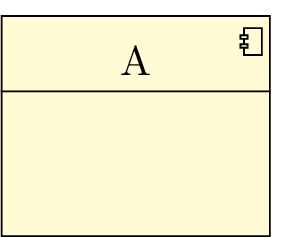
\includegraphics{fig/component.1}
\end{multicols}

Here is an example involving subitems in a component:

\begin{multicols}{2}
\begin{verbatim}
Class.A("A")()();
Package.B("B")();
Component.C("C")();

Component.BigC("Big Component")(A, B, C);

leftToRight(10)(A, B);
topToBottom(10)(A, C);

drawObject(BigC);
\end{verbatim}
\columnbreak
\hspace{3cm}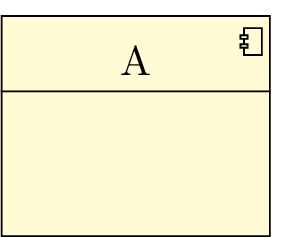
\includegraphics{fig/component.2}
\end{multicols}

\subsection{Types of Links}

\begin{tabular}{||l|c||}
\hline
{\code link(requiredInterface)( A.e -- .5[A.e, B.w] );} & 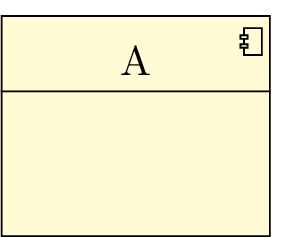
\includegraphics{fig/component.3} \\
\hline
{\code link(providedInterface)( .5[A.e, B.w] -- B.w );} & 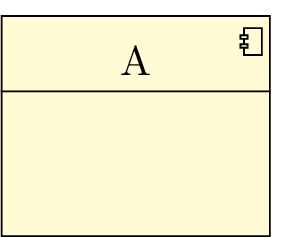
\includegraphics{fig/component.4} \\
\hline
\end{tabular}

\vspace{0.5cm}

The {\code requiredInterface} and {\code providedInterface} visual constructs can be easily combined, as shown in the following example:

\begin{multicols}{2}
\begin{verbatim}
Component.A("A")();
Component.B("B")();

leftToRight(80)(A, B);

drawObjects(A, B);

link(providedInterface)( A.e -- .5[A.e, B.w] );
link(requiredInterface)( B.w -- .5[A.e, B.w] );
\end{verbatim}
\columnbreak
\hspace{-1cm}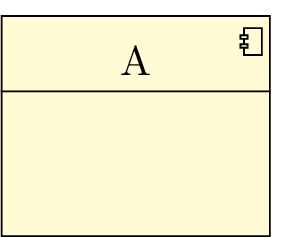
\includegraphics{fig/component.5}
\end{multicols}


\section{Use Case Diagrams}

\subsection{Use Cases}
An use case is created by the macro {\code Usecase}:

\begin{verbatim}
Usecase.name(list-of-lines);
\end{verbatim}

The {\code list-of-lines} is a comma-separated list of strings. These strings are placed
on top of each other, centered and surrounded by the appropriate visual UML notation.

Here is an use case example:

\begin{multicols}{2}
\begin{verbatim}
Usecase.U("Authenticate user",
          "by name, password");
drawObject(U);
\end{verbatim}
\columnbreak
\hspace{1cm}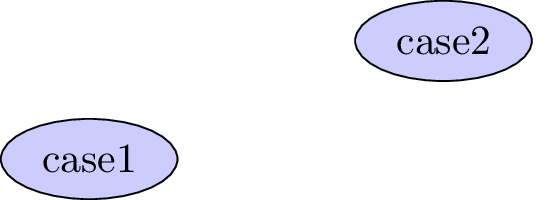
\includegraphics{fig/usecase.1}
\end{multicols}

\subsection{Actors}

An actor is created by the macro {\code Actor}:

\begin{verbatim}
Actor.name(list-of-lines);
\end{verbatim}

Here, {\code list-of-lines} represents the actor's name. For convenience, the name may be
given as a list of strings which are placed on top of each other, to provide support for
the situations when the role is quite long. Otherwise, giving a single string
as an argument to the Actor constructor is perfectly fine.

Here is an actor example:

\begin{multicols}{2}
\begin{verbatim}
Actor.A("User");
drawObject(A);
\end{verbatim}
\columnbreak
\hspace{1cm}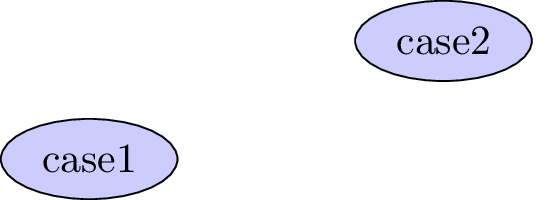
\includegraphics{fig/usecase.2}
\end{multicols}

Sometimes it may be preferable to draw diagram relations positioned relatively to
the visual representation of an actor (the ``human'') rather than relatively to the whole
actor object (which also includes the text). Because of that, MetaUML provides access
to the ``human'' of every actor object {\code actor} by means of the sub-object {\code actor.human}.

\begin{multicols}{2}
\begin{verbatim}
Actor.A("Administrator");
drawObject(A);
draw objectBox(A);
draw objectBox(A.human);
\end{verbatim}
\columnbreak
\hspace{1cm}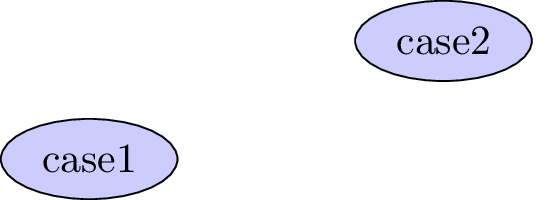
\includegraphics{fig/usecase.3}
\end{multicols}

In MetaUML, {\code objectBox(X)} is equivalent to {\code X.nw -- X.ne -- X.se -- X.sw -- cycle} for every object {\code X}. {\code A.human} is considered a MetaUML object, so you can use expressions like {\code A.human.n} or {\code A.human.midx}.

\subsection{Types of Links}

Some of the types of links defined for class diagrams (such as inheritance, association etc.) can be used with similar semantics within use case diagrams.

\section{Activity Diagrams}

\subsection{Begin, End and Flow End}

The begin and the end of an activity diagram can be marked by using the macros {\code Begin}
and {\code End} or {\code FlowFinal}, respectively. The constructors of these visual objects take no parameters:

\begin{verbatim}
Begin.beginName;
End.endName;
\end{verbatim}

Below is an example:

\begin{multicols}{2}
\begin{verbatim}
Begin.b;
End.e;
FlowFinal.f;

leftToRight(20)(b, e, f);

drawObjects(b, e, f);
\end{verbatim}
\columnbreak
\hspace{1cm}\includegraphics{fig/activity.1}
\end{multicols}

\subsection{Activity}

An activity is constructed as follows:
\begin{verbatim}
Activity.name(list-of-strings);
\end{verbatim}

The parameter {\code list-of-strings} is a comma-separated list of strings. These strings are
centered on top of each other to allow for the accommodation of a longer activity description
within a reasonable space.

An example is given below:

\begin{multicols}{2}
\begin{verbatim}
Activity.A("Learn MetaUML -",
           "the MetaPost UML library");
drawObject(A);
\end{verbatim}
\columnbreak
\hspace{1cm}\includegraphics{fig/activity.2}
\end{multicols}

\subsection{Fork and Join}

A fork or join is created by the macro:

\begin{verbatim}
Fork.name(type, length);
\end{verbatim}

The parameter {\code type} is a string and can be either of {\code "h"}, {\code "horiz"}, {\code "horizontal"}
for horizontal bars, and either of {\code "v"}, {\code "vert"}, {\code "vertical"} for vertical bars.
The {\code length} gives the bar's length.

\begin{multicols}{2}
\begin{verbatim}
Fork.forkA("h", 100);
Fork.forkB("v", 20);

leftToRight(10)(forkA, forkB);

drawObject(forkA, forkB);
\end{verbatim}
\columnbreak
\hspace{1cm}\includegraphics{fig/activity.3}
\end{multicols}

\subsection{Branch}

A branch is created by the macro:

\begin{verbatim}
Branch.name;
\end{verbatim}

Here is an example:

\begin{multicols}{2}
\begin{verbatim}
Branch.testA;

drawObject(testA);
\end{verbatim}
\columnbreak
\hspace{1cm}\includegraphics{fig/activity.4}
\end{multicols}


\subsection{Types of Links}

In activity diagrams, transitions between activities are needed. They are typeset
as in the example below. In section \ref{composite-states} such a transition
is showed. This type of link is also used for state machine diagrams.

\begin{verbatim}
link(transition)( pointA -- pointB );
\end{verbatim}

\section{State Diagrams}

The constructor of a state allows for aggregated sub-states:

\begin{verbatim}
State.name(state-name)(substates-list);
\end{verbatim}

The parameter {\code state-name} is a string or a list of comma-separated strings representing
the state's name or description. The {\code substates-list} parameter is used to specify
the substates of this state as a comma-separated list of objects; this list may be void.

An example of a simple state:

\begin{multicols}{2}
\begin{verbatim}
State.s("Take order")();
drawObject(s);
\end{verbatim}
\columnbreak
\hspace{1cm}\includegraphics{fig/state.1}
\end{multicols}


\subsection{Composite States}
\label{composite-states}

A composite state is defined by enumerating at the end of its constructor the inner
states. Interestingly enough, the composite state takes care of drawing the sub-states it
contains. The transitions must be drawn after the composite state, as seen in the
next example:

\begin{multicols}{2}
\begin{verbatim}
Begin.b;
End.e;
State.c("Component")();
State.composite("Composite")(b, e, c);

b.midx = e.midx = c.midx;
c.top = b.bottom - 20;
e.top = c.bottom - 20;

composite.info.drawNameLine := 1;
drawObject(composite);

link(transition)(b.s -- c.n);
link(transition)(c.s -- e.n);
\end{verbatim}
\columnbreak
\hspace{1cm}\includegraphics{fig/state.2}
\end{multicols}

\subsection{Internal Transitions}

Internal transitions can be specified by using the macro:
\begin{verbatim}
stateTransitions.name(list-transitions);
\end{verbatim}

Identifier {\code name} gives the state object whose internal transitions are being set,
and parameter {\code list-transitions} is a comma-separated string list.


An example is given below:

\begin{multicols}{2}
\begin{verbatim}
State.s("An interesting state",
        "which is worth mentioning")();
stateTransitions.s(
  "OnEntry / Open eyes",
  "OnExit  / Sleep well");
s.info.drawNameLine := 1;

drawObject(s);
\end{verbatim}
\columnbreak
\hspace{1cm}\includegraphics{fig/state.3}
\end{multicols}

\subsection{Special States}

Similarly to the usage of {\code Begin} and {\code End} macros, one can define history states,
exit/entry point states and terminate pseudo-states, by using the following constructors.

\begin{verbatim}
History.nameA;
ExitPoint.nameB;
EntryPoint.nameC;
Terminate.nameD;
\end{verbatim}

\section{Drawing Paths}

The {\code link} macro is powerful enough to draw relations following arbitrary paths:

\begin{multicols}{2}
\begin{verbatim}
path cool;
cool := A.e .. A.e+(20,10) ..
        B.s+(20,-40) .. B.s+(-10,-30)
        -- B.s;
link(inheritance)(cool);

link(aggregationUni)
    (A.n ..(30,30)..B.w);
\end{verbatim}
\columnbreak
\hspace{1cm}\includegraphics{fig/paths.1}
\end{multicols}

Amusing as it may be, this feature gets old soon. When typesetting UML diagrams in good style, rectangular paths are usually preferred. 
It is for this kind of paths that MetaUML offers extensive support, by means of ``syntactic sugar'' constructs which
are not only self-documenting, but reduce the amount of typing and thinking required.

\subsection{Manhattan Paths}

The ``Manhattan'' path macros generate a path between two points consisting of one
horizontal and one vertical segment. The macro {\code pathManhattanX} generates first a
horizontal segment, while the macro {\code pathManhattanY} generates first a
vertical segment. In MetaUML it also matters the direction of a path, so you
can choose to reverse it by using {\code rpathManhattanX} and {\code rpathManhattanY}
(note the prefix ``{\code r}''):

\begin{verbatim}
pathManhattanX(A, B)
pathManhattanY(A, B)

rpathManhattanX(A, B)
rpathManhattanY(A, B)
\end{verbatim}

\pagebreak
Here is an example:

\begin{multicols}{2}
\begin{verbatim}
Class.A("A")()();
Class.B("B")()();

B.sw = A.ne + (10,10);
drawObjects(A, B);

link(aggregationUni)
   (rpathManhattanX(A.e, B.s));
link(inheritance)
   (pathManhattanY(A.n, B.w));
\end{verbatim}
\columnbreak
\hspace{1cm}\includegraphics{fig/paths.2}
\end{multicols}

\subsection{Stair Step Paths}

These path macros generate stair-like paths between two points.
The ``stair'' can ``rise'' first in the direction of $Ox$ axis ({\code pathStepX})
or in the direction of $Oy$ axis ({\code pathStepY}). How much should a step
rise is given by an additional parameter, {\code delta}. Again, the macros
prefixed with ``{\code r}'' reverse the direction of the path given by their
unprefixed counterparts.

\begin{verbatim}
pathStepX(A, B, delta)
pathStepY(A, B, delta)

rpathStepX(A, B, delta)
rpathStepY(A, B, delta)
\end{verbatim}

Here is an example:

\begin{multicols}{2}
\begin{verbatim}
stepX:=60;
link(aggregationUni)
   (pathStepX(A.e, B.e, stepX));

stepY:=20;
link(inheritance)
   (pathStepY(B.n, A.n, stepY));
\end{verbatim}
\columnbreak
\hspace{1cm}\includegraphics{fig/paths.3}
\end{multicols}

\subsection{Horizontal and Vertical Paths}

There are times when drawing horizontal or vertical links is required,
even when the objects are not properly aligned. To this aim, the following macros
are useful:

\begin{verbatim}
pathHorizontal(pA, untilX)
pathVertical(pA, untilY)

rpathHorizontal(pA, untilX)
rpathVertical(pA, untilY)
\end{verbatim}

A path created by {\code pathHorizonal} starts from the point {\code pA}
and continues horizontally until coordinate {\code untilX} is reached. The macro
{\code pathVertical} constructs the path dually, working vertically.
The prefix ``{\code r}'' reverses the direction of the path.

Usage example:

\begin{multicols}{2}
\begin{verbatim}
untilX := B.left;
link(association)
   (pathHorizontal(A.e, untilX));

untilY:= C.bottom;
link(association)
   (pathVertical(A.n, untilY));
\end{verbatim}
\columnbreak
\hspace{1cm}\includegraphics{fig/paths.4}
\end{multicols}

\subsection{Direct Paths}

A direct path can be created with {\code directPath}. The call {\code directPath(A, B)}
is equivalent to {\code A -{}-  B}.

\subsection{Paths between Objects}

Using the constructs presented above, links between diagram objects are drawn easily like this:

\begin{verbatim}
link(transition)(directPath(objA.nw, objB.se));
\end{verbatim}

There are times however when this direct approach may yield unsatisfactory visual results,
especially when the object's corners is round. To tackle these situations, MetaUML provides the macro
{\code pathCut}, whose aim is to limit a given path exactly to the region outside the actual
borders of the objects it connects. The macro's synopsis is:

\begin{verbatim}
pathCut(thePath)(objectA, objectB)
\end{verbatim}

Here, {\code thePath} is a given MetaPost path and {\code objectA} and {\code objectB}
are two MetaUML objects. By contract, each MetaUML object of type, say, {\code X}
defines a macro {\code X\_border} which returns the path that surrounds it. Because
of that, {\code pathCut} can make the appropriate modifications to {\code thePath}.

The following code demonstrates the benefits of the {\code pathCut} macro:

\begin{multicols}{2}
\begin{verbatim}
z = A.se + (30, -10);
link(transition)
   (pathCut(A, B)(A.c--z--B.c));
\end{verbatim}
\columnbreak
\hspace{1cm}\includegraphics{fig/paths.5}
\end{multicols}

\subsubsection{Direct Paths between Centers}

At times is quicker to just draw direct paths between the center of two objects,
minding of course the object margins. The macro which does this is {\code clink}:

\begin{verbatim}
clink(how-to-draw-information)(objA, objB);
\end{verbatim}

The parameter {\code how-to-draw-information} is the same as for the macro {\code link};
{\code objA} and {\code objB} are two MetaUML objects.

Below is an example which involves the inheritance relation:

\begin{multicols}{2}
\begin{verbatim}
clink(inheritance)(A, B);
\end{verbatim}
\columnbreak
\hspace{1cm}\includegraphics{fig/paths.6}
\end{multicols}

\section{Arranging Diagram Items}
\label{section:positioning}

Using equations involving cardinal points, such as {\code A.nw = B.ne + (10,0)}, is
good enough for achieving the desired results. However, programs are best to
be written for human audience, rather than for compilers. It does become a bit
tiresome to think all the time of cardinal points and figure out the
direction of positive or negative offsets. Because of that, MetaUML offers
syntactic sugar which allows for an easier understanding of the intent behind
the positioning code.

Suppose that we have three classes, {\code A}, {\code B}, {\code C} and their base class
{\code Base}. We want the base class to be at the top, and the derived classes to be
on a line below. This code will do:

\begin{verbatim}
A.ne = B.nw + (20,0);
B.ne = C.nw + (20,0);
Base.s = B.n + (0,-20);
\end{verbatim}

Unfortunately, writing code such as this makes it hard for fellow programmers to visualize
its intent upon reading it. And ``fellow programmers`` include the author, five minutes later.

Perhaps the next version of the code will drive home the point. The outcome is
the same as before, but the layout is stated in a more human-friendly way. You might even
infer by yourself that the numeric argument represents the distance between the objects.

\begin{multicols}{2}
\begin{verbatim}
leftToRight(20)(A, B, C);
topToBottom(20)(Base, B);
\end{verbatim}
\columnbreak
\hspace{1cm}\includegraphics{fig/positioning.2}
\end{multicols}

Below there are examples which show how these macros can be used. Suppose that we have the 
following definitions for objects {\code X}, {\code Y}, and {\code Z}; also, let's assume 
that {\code spacing} is a numeric variable set to {\code 5}.

\begin{verbatim}
Picture.X("a");
Picture.Y("...");
Picture.Z("Cyan");
\end{verbatim}

\begin{tabular}{||l|c||}
\hline
{\code leftToRight.top(spacing)(X, Y, Z);} & \includegraphics{fig/positioning.3} \\
\hline
{\code leftToRight.midy(spacing)(X, Y, Z);} & \includegraphics{fig/positioning.4} \\
\hline
{\code leftToRight.bottom(spacing)(X, Y, Z);} & \includegraphics{fig/positioning.5} \\
\hline
{\code topToBottom.left(spacing)(X, Y, Z);} & \includegraphics{fig/positioning.6} \\
\hline
{\code topToBottom.midx(spacing)(X, Y, Z);} & \includegraphics{fig/positioning.7} \\
\hline
{\code topToBottom.right(spacing)(X, Y, Z);} & \includegraphics{fig/positioning.8} \\
\hline
\end{tabular} \\

To make things even easier, the following equivalent contructs are also allowed:

\begin{verbatim}
leftToRight.midy(spacing)(X, Y, Z);
leftToRight(spacing)(X, Y, Z);
\end{verbatim}

\begin{verbatim}
topToBottom.midx(spacing)(X, Y, Z);
topToBottom(spacing)(X, Y, Z);
\end{verbatim}

If you want to specify that some objects have a given property equal, while the distance between them is given elsewhere, you can use the macro {\code same}.
This macro accepts a variable number of parameters, but at least two. The following table gives the interpretation of the macro for a simple example.

\begin{tabular}{||l|l||}
\hline
{\code same.top(X, Y, Z);} & {\code X.top = Y.top = Z.top;} \\
\hline
{\code same.midy(X, Y, Z);} & {\code X.midy = Y.midy = Z.midy;} \\
\hline
{\code same.bottom(X, Y, Z);} & {\code X.bottom = Y.bottom = Z.bottom;} \\
\hline
{\code same.left(X, Y, Z);} & {\code X.left = Y.left = Z.left;} \\
\hline
{\code same.midx(X, Y, Z);} & {\code X.midx = Y.midx = Z.midx;} \\
\hline
{\code same.right(X, Y, Z);} & {\code X.right = Y.right = Z.right;} \\
\hline
\end{tabular} \\

Relative positions of two points can be declared more easily using the macros {\code below}, {\code above}, {\code atright}, {\code atleft}.
Let us assume that {\code A} and {\code B} are two points (objects of type {\code pair} in MetaPost). The following constructs are equivalent:

\begin{tabular}{||l|l||}
\hline
{\code B = A + (5,0);} & {\code B = atright(A, 5);} \\
{\code B = A - (5,0);} & {\code B = atleft(A, 5);} \\
{\code B = A + (0,5);} & {\code B = above(A, 5);} \\
{\code B = A - (0,5);} & {\code B = below(A, 5);} \\
\hline
\end{tabular}


\section{The MetaUML Infrastructure}
\label{section:infrastructure}

MetaPost is a macro language based on equation solving. Using it may seem quite
tricky at first for a programmer accustomed to modern object-oriented languages.
However, the great power of MetaPost consists in its versatility. Indeed, it is possible to write
a system which mimics quite well object-oriented behavior. Along this line, METAOBJ
\cite{metaobj} is a library worth mentioning: it provides a high-level objects
infrastructure along with a battery of predefined objects.

Surprisingly enough, MetaUML does not use METAOBJ. Instead, it uses a custom written,
lightweight object-oriented infrastructure, provisionally called ``{\code util}''.
METAOBJ's facilities, although impressive, were perceived by me as being a bit too much
for what was initially intented as a quick way of getting some UML diagrams layed out.
Inspired by METAOBJ, ``{\code util}'' was designed to fulfill with minimal effort
the specific tasks needed to confortably position, allign or group visual objects
which include text.

Another library having some object-oriented traits is the {\code boxes}
library, which comes with the standard MetaPost distribution. Early versions of
MetaUML did use {\code boxes} as an infrastructure, but this approach had to be abandoned eventually.
The main reason was that it was difficult to achieve good visual results when stacking texts
(more on that further on). For all it's worth, it did not fit well with the way in which MetaUML's
layout mechanism was shaping up at the time.

\subsection{Motivation}

Suppose that we want to typeset two texts with their bottom lines aligned, using {\code boxit}:

\begin{multicols}{2}
\begin{verbatim}
boxit.a ("yummy");
boxit.b ("cool");

a.nw = (0,0); b.sw = a.se + (10,0);

drawboxed (a, b); % or drawunboxed(a,b)
draw a.sw -- b.se dashed evenly
   withpen pencircle scaled 1.1;
\end{verbatim}
\columnbreak
\hspace{1cm}\includegraphics{fig/boxes_vs_util.1}
\end{multicols}

Note that, despite supposedly having their bottom lines alligned,
``yummy'' {\it looks} slightly higher than ``cool''. This would be unacceptable
in a UML class diagram, when roles are placed at the ends of a horizontal association.
Regardless of the default spacing being smaller in the {\code util} library,
the very same unfortunate misalignment effect rears its ugly head:

\begin{multicols}{2}
\begin{verbatim}
Picture.a("yummy");
Picture.b("cool");
% comment next line for unboxed
a.info.boxed := b.info.boxed := 1;

b.sw = a.se + (10,0);

drawObjects(a, b);
\end{verbatim}
\columnbreak
\hspace{1cm}\includegraphics{fig/boxes_vs_util.2}
\end{multicols}

However, the strong point of {\code util} is that we have a recourse to this problem:

\begin{multicols}{2}
\begin{verbatim}
iPict.ignoreNegativeBase := 1;

Picture.a("yummy");
Picture.b("cool");
% the rest the same as above
drawObjects(a, b);
\end{verbatim}
\columnbreak
\hspace{1cm}\includegraphics{fig/boxes_vs_util.3}
\end{multicols}

\subsection{The Picture Macro}

We have seen previously the line {\code iPict.ignoreNegativeBase := 1}.
Who is {\code iPict} and what is it doing in our program? MetaUML
aims at separating the ``business logic'' (what to draw) from the
``interface'' (how to draw). In order to achieve this, it records the ``how to draw''
information within the so-called {\code Info} structures. The object {\code iPict}
is an instance of {\code PictureInfo} structure, which has the following properties
(or attributes):
\begin{verbatim}
left, right, top, bottom
ignoreNegativeBase
boxed, borderColor
\end{verbatim}

The first four attributes specify how much space should be left around the
actual item to be drawn. The marvelous effect of {\code ignoreNegativeBase}
has just been shown (off), while the last two attributes control whether the border
should be drawn (when {\code boxed=1}) and if drawn, in which color.

There's one more thing: the font to typeset the text in. This is specified
in a {\code FontInfo} structure which has two attributes: the font name
and the font scale. This information is kept within the {\code PictureInfo} structure
as a contained attribute {\code iFont}. Both {\code FontInfo} and {\code PictureInfo}
have ``copy constructors'' which can be used to make copies. We have already
the effect of these copy constructors at work, when we used:

\begin{verbatim}
Picture.a("yummy");
a.info.boxed := 1;
\end{verbatim}

A copy of the default info for a picture, {\code iPict}, has been made within
the object {\code a} and can be accessed as {\code a.info}. Having a copy of the
info in each object may seem like an overkill, but it allows for a fine grained
control of the drawing mode of each individual object. This feature comes in very
handy when working with a large number of settings, as it is the case for MetaUML.

Let us imagine for a moment that we have two types of text to write: one with a small font
and a small margin and one with a big font and a big margin. We could in theory
configure each individual object or set back and forth global parameters, but
this is far for convenient. It is preferable to have two sets of settings and specify
them explicitly when they are needed. The following code could be placed somewhere
in a configuration file and loaded before any {\code beginfig} macro:
\begin{verbatim}
PictureInfoCopy.iBig(iPict);
iBig.left := iBig.right := 20;
iBig.top := 10;
iBig.bottom := 1;
iBig.boxed := 1;
iBig.ignoreNegativeBase := 1;
iBig.iFont.name := defaultfont;
iBig.iFont.scale := 3;

PictureInfoCopy.iSmall(iPict);
iSmall.boxed := 1;
iSmall.borderColor := green;
\end{verbatim}

Below is an usage example of these definitions. Note the name of the macro: {\code EPicture}.
The prefix comes form ``explicit''  and it's used to acknowledge that the
``how to draw'' information is given explicitly --- as a parameter,
rather than defaulted to what's recorded in {\code iPict}, as with the {\code Picture} macro.
Having predefined configurations yields short, convenient code.

\begin{multicols}{2}
\begin{verbatim}
EPicture.a(iBig)("yummy");
EPicture.b(iSmall)("cool");
% you can still modify a.info, b.info

b.sw = a.se + (10,0);

drawObjects(a, b);
\end{verbatim}
\columnbreak
\hspace{1cm}\includegraphics{fig/picture_info.1}
\end{multicols}

\subsubsection{Fixed Sizes}

By default, the size of a {\code Picture} object is set by its contents. However,
it is possible to specify fixed dimensions both the width and the height, independently.
This can be done by setting the {\code info}'s attributes {\code fixedWidth} and {\code fixedHeight} to values
greater than 0. If any of these attributes is left to its default value, {\code -1}, then for the corresponding
axis the dimension is set according to the dimension of the content. Nevertheless, the fixed dimensions are enforced, even though the contained object would have needed additional space.

\begin{multicols}{2}
\begin{verbatim}
PictureInfoCopy.myFixed(iPict);
myFixed.ignoreNegativeBase := 1;
myFixed.fixedWidth  := 15;
myFixed.fixedHeight := 20;
myFixed.boxed := 1;

EPicture.a(myFixed)("a");
EPicture.b(myFixed)(".-.");
EPicture.c(myFixed)("toolong");

leftToRight.bottom(10)(a, b, c);

drawObjects(a, b, c);
\end{verbatim}
\columnbreak
\hspace{1cm}\includegraphics{fig/picture_info.2}
\end{multicols}

\subsubsection{Content alignment}

When fixed dimensions are used, one most likely would prefer a centered alignement of the contents in the 
{\code Picture} box. This option can be expressed independently for each of the axes, 
by setting the {\code info}'s attributes {\code valign} and {\code halign} to descriptive string values. 
For horizontal alignement, {\code halign} can be set to {\code "left"} or {\code "center"}, and for
vertical alignement, {\code valign} can be set to {\code "bottom} or {\code "center"}. The default
values for these attributes are {\code "left"} and {\code "bottom"}, respectively.

The next example uses horizontal centered alignement and a bottom alignement with a {\code 4.5} base offset, for
vertical alignement. This vertical alignement gives a better visual result than the centered one, at
least for the situations in which there are texts to be placed horizontally.

\begin{multicols}{2}
\begin{verbatim}
PictureInfoCopy.myFixed(iPict);
myFixed.ignoreNegativeBase := 1;
myFixed.bottom := 4.5;
myFixed.valign := "bottom";
myFixed.halign := "center";
myFixed.fixedWidth  := 25;
myFixed.fixedHeight := 15;
myFixed.boxed := 1;

EPicture.a(myFixed)("a");
EPicture.b(myFixed)("yum");
EPicture.c(myFixed)("b");

leftToRight.bottom(10)(a, b, c);

drawObjects(a, b, c);
\end{verbatim}
\columnbreak
\hspace{1cm}\includegraphics{fig/picture_info.3}
\end{multicols}

\subsection{Stacking Objects}

It is possible to stack objects, much in the style of {\code setboxjoin}
from {\code boxes} library.

\begin{multicols}{2}
\begin{verbatim}
Picture.a0("yummy");
Picture.a1("cool");
Picture.a2("fool");

setObjectJoin(pa.sw = pb.nw);
joinObjects(scantokens listArray(a)(3));

drawObjects(scantokens listArray(a)(3));
% or drawObjects (a0, a1, a2);
\end{verbatim}
\columnbreak
\hspace{1cm}\includegraphics{fig/object_stack.1}
\end{multicols}

The {\code listArray} macro provides here a shortcut for writing
{\code a0, a1, a2}. This macro is particularly useful for generic
code which does not know beforehand the number of elements to be drawn.
Having to write the {\code scantokens} keyword is admittedly a nuisance, but
this is required.


\subsection{The Group Macro}

It is possible to group objects in MetaUML. This feature is the cornerstone
of MetaUML, allowing for the easy development of complex objects, such as
composite stats in state machine diagrams.

Similarly to the macro {\code Picture}, the structure {\code GroupInfo}
is used for specifying group properties; its default instantiation is
{\code iGroup}. Furthermore, the macro {\code EGroup} explicitely sets the
layout information.

Here is an example:

\begin{multicols}{2}
\begin{verbatim}
iGroup.left:=20;
iGroup.right:=15;
iGroup.boxed:=1;
iPicture.boxed:=1;

Picture.a("yummy");
Picture.b("cool");
Picture.c("fool");

b.nw = a.nw + (20,20);  % A
c.nw = a.nw + (15, 40); % B

Group.g(a, b, c);
g.nw = (10,10); % C

drawObject(g);
\end{verbatim}
\columnbreak
\hspace{1cm}\includegraphics{fig/group.1}
\end{multicols}

After some objects are grouped, they can only be drawn
by invoking the {\code drawObject} macro on the group that aggregates them, and not individually.
Conveniently, once the relative positioning of objects within a group is set (line A and B), the whole
group can be ``moved'' do the desired position (line C), and all the contained objects will move along.

\subsection{The PictureStack Macro}

The {\code PictureStack} macro is a syntactic sugar for a set of pictures,
stacked according to predefined equations and grouped together.

\begin{multicols}{2}
\begin{verbatim}
iStack.boxed := 1;
iStack.iPict.boxed := 1;
PictureStack.myStack("foo",
  "bar: int" infont "tyxtt",
  "nicely-centered" infont defaultfont,
  "nice")("vcenter");

drawObject(myStack);
\end{verbatim}
\columnbreak
\hspace{1cm}\includegraphics{fig/picture_stack.1}
\end{multicols}

Note the last parameter of the macro {\code PictureStack}, here {\code vcenter}.
It is used to generate appropriate equations based on a descriptive name.
The spacing between individual picture objects is set by the field
{\code iStack.spacing}. Currently, the following alignment names are
defined: {\code vleft}, {\code vright}, {\code vcenter},
{\code vleftbase}, {\code vrightbase}, {\code vcenterbase}. All these
names refer to vertical alignment (the prefix ``{\code v}''); alignment can
be at left, right or centered. The variants having the suffix ``{\code base}'' align
the pictures so that {\code iStack.spacing} refer to the distance between the
bottom lines of the pictures. The unsuffixed variants use {\code iStack.spacing} as
the distance between one's bottom line and the next's top line.

The ``{\code base}'' alignment is particularly useful for stacking text, since it
offers better visual appearance when {\code iPict.ignoreNegativeBase} is set to {\code 1}.

\section{Components Design}

Each MetaUML component (e.g. {\code Picture}, {\code PictureStack}, {\code Class}) is
designed according to an established pattern. This section gives more insight
on this.

In order to draw a component, MetaUML categorizes the required information as follows:
\begin{itemize}
\item what to draw, or what are the elements of a component.
\item how to draw, or how are the elements positioned in relation to each other within the component
\item where to draw
\end{itemize}

For example, in order to draw a picture object we must know, respectively:
\begin{itemize}
\item what is the text or the native picture that needs to be drawn
\item what are the margins that should be left around the contents
\item where is the picture to be drawn
\end{itemize}

Why do we bother with these questions? Why don't we just simply draw the picture
component as soon as it was created and get it over with?
That is, why doesn't the following code just work?

\begin{verbatim}
Picture.pict("foo");
\end{verbatim}

Well, although we have the answer to question 1 (what to draw),
we still need to have question 3 answered. The code below becomes thus a
necessity (actually, you are not forced to specify the positioning of an object,
because its draw method positions it to {\code (0,0)} by default):

\begin{verbatim}
% question 1: what to draw
Picture.pict("foo");

% question 3: where to draw
pict.nw = (10,10);

% now we can draw
drawObject(pict);
\end{verbatim}

How about question 2, how to draw? By default, this problem is addressed behind the
scenes by the component. This means, for the Picture object, that a native picture is created
from the given string, and around that picture certain margins are placed, by means of MetaPost equations.
(The margins also come in handy when stacking Picture objects, so that the result doesn't look too cluttered.)
If these equations were defined within the Picture constructor, then an
usability problem would have appeared, because it wouldn't have been possible to modify the margins,
as in the code below:

\begin{verbatim}
% question 1: what to draw
Picture.pict("foo");

% question 2: how to draw
pict.info.left := 10;
pict.info.boxed := 1;

% question 3: where to draw
pict.nw = (0,0);

% now we can draw
drawObject(pict);
\end{verbatim}

To allow for this type of code, the equations that define the layout of the {\code Picture} object (here, what the margins are)
must be defined somewhere after the constructor. This is done by a macro called {\code Picture\_layout}.
This macro defines all the equations which link the ``what to draw'' information to the ``how to draw''
information (which in our case is taken from the {\code info} member, a copy of {\code iPict}).
Nevertheless, notice that {\code Picture\_layouts} is not explicitly invoked. To the user's
great relief, this is taken care of automatically within the {\code Picture\_draw} macro.

There are times however, when explicitly invoking a macro like {\code Picture\_layout}
becomes a necessity. This is because, by contract, it is only after the {\code layout}
macro is invoked that the final dimensions (width, height) of an object are
definitely and permanently known. Imagine that we have a component whose job is to
surround in a red-filled rectangle some other objects. This component
needs to know what the dimensions of the contained objects are, in order to be able to set
its own dimensions. At drawing time, the contained objects must not have been drawn already,
because the red rectangle of the container would overwrite them.
Therefore, the whole pseudo-code would be:
\begin{verbatim}
Create objects o1, o2, ... ok;
Create container c(o1, o2, ..., ok);
Optional: modify info-s for o1, o2, ... ok;
Optional: modify info for c;

layout c, requiring layout of o1, o2, ... ok;
establish where to draw c;
draw red rectangle defined by c;
draw components o1, o2, ...ok within c
\end{verbatim}

A natural conclusion is that an object must not be laid out more than once, because otherwise
inconsistent or superfluous equations would arise. To enforce this, by contract,
any object must keep record of whether its layout method has already been invoked,
and if the answer is affirmative, subsequent invocations of the layout macro would
do nothing. It is very important to mention that after the {\code layout} macro is
invoked over an object, modifying the {\code info} member of that object has
no subsequent effect, since the layout equations are declared and interpreted only once.

\subsection{Notes on the Implementation of Links}

MetaUML considers edges in diagram graphs as links. A link is composed of a path and the
heads (possible none, one or two). For example, since an association has no heads, it suffices 
to draw along the path with a solid pen; however, an unidirectional aggregation has, in addition 
to a solid path, two heads: one is an arrow and the other is a diamond.

The general algorithm for drawing a link is:

\begin{verbatim}
0. Reserve space for heads
1. Draw the path (except for the heads)
2. Draw head 1
3. Draw head 2
\end{verbatim}

Each of the UML link types define how the drawing should be done, in each of the
cases (1, 2 and 3). Consider the link type of unidirectional composition.
Its ``class'' is declared as:

\begin{verbatim}
vardef CompositionUniInfo@# =
  LinkInfo@#;

  @#widthA      = defaultRelationHeadWidth;
  @#heightA     = defaultRelationHeadHeight;
  @#drawMethodA = "drawArrow";

  @#widthB      = defaultRelationHeadWidth;
  @#heightB     = defaultRelationHeadHeight;
  @#drawMethodB = "drawDiamondBlack";

  @#drawMethod = "drawLine";
enddef;
\end{verbatim}

Using this definition, the actual description is created like this:

\begin{verbatim}
CompositionUniInfo.compositionUni;
\end{verbatim}

As shown previously, is is the macro {\code link} which
performs the actual drawing, using the link description information
which is given as parameter (generally called {\code iLink}).
For example, we can use:

\begin{verbatim}
link(aggregationUni)((0,0)--(40,0));
\end{verbatim}

%\begin{figure}
%\centering
%\includegraphics{fig/how-links-work.1}
%\caption{An example of a picture stack.}
%\label{fig:hlw}
%\end{figure}

Let us see now the inner workings of macro {\code link}. Its definition is:

\begin{verbatim}
vardef link(text iLink)(expr myPath)=
   LinkStructure.ls(myPath,
                    iLink.widthA, iLink.widthB);
   drawLinkStructure(ls)(iLink);
enddef;
\end{verbatim}

\begin{figure}
\centering
\begin{tabular}{l|l}
$AB$ & the path specified by the user \\
$|AA'|$ & {\code iLink.widthA}\\
$|BB'|$ & {\code iLink.widthB}
\end{tabular}
\includegraphics{fig/how-links-work.2}
\caption{Details on how a link is drawn by MetaUML.}
\label{fig:hlw2}
\end{figure}

First, space is reserved for heads, by ``shortening'' the given path {\code myPath}
by {\code iLink.widthA} at the beginning and by {\code iLink.widthB} at the end.
After that, the shortened path is drawn with the ``method''
given by {\code iLink.drawMethod} and the heads with the ``methods''
{\code iLink.drawMethodA} and {\code iLink.drawMethodB},
respectively (figure \ref{fig:hlw2}).

\subsection{Object Definitions: Easier {\code generic\_declare}}

In MetaPost, if somebody wants to define something resembling a class in an object-oriented language,
named, say, {\code Person}, he would do something like this:

\begin{verbatim}
vardef Person@#(expr _name, _age)=
  % @# prefix can be seen as `this` pointer
  string @#name;
  numeric @#age;

  @#name := _name;
  @#age := _age;
enddef;
\end{verbatim}

This allows for the creation of instances (or objects) of class {\code Person} by using
declarations like:

\begin{verbatim}
Person.personA;
Person.personB;
\end{verbatim}

 However, if one also wants to able able to create indexed arrays of persons, such as
{\code Person.student0}, {\code Person.student1} etc., the definition of class
{\code Person} must read:

\begin{verbatim}
vardef Person@#(expr _name, _age)=
  _n_ := str @#;
  generic_declare(string) _n.name;
  generic_declare(numeric) _n.age;

  @#name := _name;
  @#age := _age;
enddef;
\end{verbatim}

This construction is rather inelegant. MetaUML offers alternative macros to achieve
the same effect, uncluttering the code by removing the need for the unaesthetic {\code \_n\_} and
{\code \_n}.

\begin{verbatim}
vardef Person@#(expr _name, _age)=
  attributes(@#);
  var(string) name;
  var(numeric) age;

  @#name := _name;
  @#age := _age;
enddef;
\end{verbatim}

\section{Customization in MetaUML: Examples}
\label{section:customization}

We have seen that in MetaUML the ``how to draw'' information is memorized into the so-called
``{\code Info}'' structures. For example, the default way in which a {\code Picture} object is
to be drawn is recorded into an instance of {\code PictureInfo}, named {\code iPict}. In this section we
present a case study involving the customization of {\code Class} objects. The customization of
any other MetaUML objects works similarly. Here we cannot possibly present all the customization
options for all kinds of MetaUML objects: this would take too long. Nevertheless, an interested reader can refer
to the top of the appropriate MetaUML library file, where {\code Info} structures are defined.
For example, class diagram related definitions are in {\code metauml\_class.mp}, activity diagram
definitions are in {\code metauml\_activity.mp} etc.

\subsection{Global settings}

Let us assume that we do not particularly like the default foreground color of all classes, and wish
to change it so something yellowish. In this scenario, one would most likely want to change
the appropriate field in {\code iClass}:

\begin{verbatim}
iClass.foreColor := (.9, .9, 0);
\end{verbatim}

After this, we can obtain the following result:

\begin{multicols}{2}
\begin{verbatim}
Class.A("A")()();
Class.B("B")()();
Class.C("C")()();

B.w = A.e + (20,0);
C.n = .5[A.se, B.sw] + (0, -10);

drawObjects(A, B, C);
\end{verbatim}
\columnbreak
\hspace{1cm}\includegraphics{fig/class_customization.1}
\end{multicols}

\subsection{Individual settings}

To modify the settings of one particular {\code Class} objects, another strategy is more appropriate. How about having class
{\code C} stand out with a light blue foreground color, a bigger font size for the class name and a blue border?

\begin{multicols}{2}
\begin{verbatim}
iPict.foreColor := (.9, .9, 0);

Class.A("A")()();
Class.B("B")()();
Class.C("C")()();
C.info.foreColor := (.9, .7, .7);
C.info.borderColor := green;
C.info.iName.iFont.scale := 2;

% positioning code ommited
drawObjects(A, B, C);
\end{verbatim}
\columnbreak
\hspace{1cm}\includegraphics{fig/class_customization.2}
\end{multicols}

As an aside, each {\code Class} object has an {\code info} member which is created as
a copy of {\code iClass}; the actual drawing is performed using this copied
information. Because of that, the {\code info} member can be safely modified after the object
has been created, obtaining the expected results and not influencing other objects.

Another thing worth mentioning is that the {\code ClassInfo} structure contains
the {\code iName} member, which is an instance of {\code PictureInfo}. In our example we
do not want to modify the spacings around the {\code Picture} object,
but the characteristics of the font its contents is typeset into. To do that,
we modify the {\code iName.iFont} member, which by default is a copy of {\code iFont}
(an instance of {\code FontInfo}, defined in {\code util\_picture.mp}).
If, for example, we want to change the font the class name is rendered into, we would set
the attribute {\code iName.iFont.name} to a string representing a font name
on our system (as used with the MetaPost {\code infont} operator).

\subsection{Predefined settings}

This usage scenario is perhaps more interesting. Suppose that we have two
types of classes which we want to draw differently. Making the setting adjustments
for each individual class object would soon become a nuisance. MetaUML's solution consists in the
ability of using predefined ``how to draw'' {\code Info} objects. Let us create such objects:

\begin{verbatim}
ClassInfoCopy.iHome(iClass);
iHome.foreColor := (0, .9, .9);

ClassInfo.iRemote;
iRemote.foreColor := (.9, .9, 0);
iRemote.borderColor := green;
\end{verbatim}

Object {\code iHome} is a copy of {\code iClass} (as it might have been set at
the time of the macro call). Object {\code iRemote} is created just as {\code iClass}
is originally created. We can now use these {\code Info} objects to easily set the
``how to draw'' information for classes. The result is depicted below,
please note the ``{\code E}'' prefix in {\code EClass}:

\begin{multicols}{2}
\begin{verbatim}
EClass.A(iHome)("UserHome")()();
EClass.B(iRemote)("UserRemote")()();
EClass.C(iHome)("CartHome")()();
EClass.D(iRemote)("CartRemote")()();
\end{verbatim}
\columnbreak
\hspace{1cm}\includegraphics{fig/class_customization.3}
\end{multicols}

\subsection{Extreme customization}

When another font (or font size) is used, it may become necessary to change the space between the
baselines of attributes and methods. Figure below is the result of the (unlikely) code:

\begin{multicols}{2}
\begin{verbatim}
Class.A("Foo")
  ("a: int", "b: int")
  ("foo()", "bar()", "gar()");

A.info.iName.iFont.name := metauml_defaultFontBold;
A.info.iName.iFont.scale := 1.2;

A.info.iAttributeStack.iPict.iFont.scale := 0.8;
A.info.iAttributeStack.top := 10;
A.info.iAttributeStack.spacing := 11;

A.info.iMethodStack.iPict.iFont.scale := 2;
A.info.iMethodStack.spacing := 17;
A.info.iMethodStack.bottom := 10;

drawObject(A);
\end{verbatim}
\columnbreak
\hspace{4cm}\includegraphics{fig/class_customization.4}
\end{multicols}

\begin{verbatim}
\end{verbatim}

Both {\code iAttributeStack} and {\code iMethodStack} are instances of
{\code PictureStackInfo}, which is used to control the display of {\code PictureStack} objects.
%We can also customize the size and colors of the ``locks'' by setting {\code A.info.iLock}.

As font names, you can choose from the globally defined {\code metauml\_defaultFont}, {\code metauml\_defaultFontOblique}, {\code metauml\_defaultFontBold}, {\code metauml\_defaultFontBoldOblique}, or any other name of a font that is available on your system.

\section{Alternatives to MetaUML}

No software package is perfect, and for this MetaUML is a prime example. Here is a list of packages that may also be used to create UML diagrams for LaTeX work:

\begin{itemize}
\item uml.sty \cite{umlsty}
\item pst-uml \cite{pstumlsty}
\item umldoc \cite{umldoc}
\item TiKZ-UML \cite{tikzuml}
\end{itemize}

Do not ignore the possibility of creating your diagrams using a GUI program, and then exporting them into a LaTex-friendly open format such as SVG \cite{svglatex}.

\pagebreak
%    Part of the MetaUML manual
%    Copyright (c) 2005 Ovidiu Gheorghies
%
%    Permission is granted to copy, distribute and/or modify this document
%    under the terms of the GNU Free Documentation License, Version 1.2
%    or any later version published by the Free Software Foundation;
%    with no Invariant Sections, no Front-Cover Texts, and no Back-Cover Texts.
%    A copy of the license is included in the section entitled "GNU
%    Free Documentation License".

\newcommand{\metaumltest}[2]{Test #2 --- \\ \includegraphics{fig/test_#1.#2} \\ }
\newcommand{\metaumltests}[2]{\multido{\iA=1+1}{#2}{\metaumltest{#1}{\iA}}} 

\section{Test Suite}

\subsection{Low-level}
  \metaumltests{lowlevel}{2}

\subsection{Fonts}
  \metaumltests{font}{3}

\subsection{Util library}
  \subsubsection{Picture tests}
    \metaumltests{picture}{10}

  \subsubsection{Picture tests - TeX rendering}
    \metaumltests{picture_tex_rendering}{1}

  \subsubsection{Group tests}
    \metaumltests{group}{2}

  \subsubsection{PictureStack tests}
    \metaumltests{picture_stack}{7}

  \subsubsection{Positioning tests}
    \metaumltests{positioning}{6}

\subsection{Class diagram}
  \subsubsection{Class tests}
    \metaumltests{class}{16}
  \subsubsection{Class feature types tests}
    \metaumltests{class_feature_types}{5}
  \subsubsection{Class template tests}
    \metaumltests{class_templates}{3}

  \subsubsection{Qualified Association tests}
    \metaumltests{class_qual_assoc}{2}
    
\subsection{Package diagram}
\subsubsection{Package tests}
    \metaumltests{package}{2}

\subsection{Component diagram}
\subsubsection{Component tests}
    \metaumltests{component}{1}

\subsection{Paths}
  \metaumltests{paths}{3}

\subsection{Behavioral diagrams}
  \subsubsection{Activity tests}
    \metaumltests{activity}{2}

  \subsubsection{State Machine tests}
    \metaumltests{state}{5}

  \subsubsection{Usecase tests}
    \metaumltests{usecase}{9}

\subsection{Miscelaneous}
  \subsubsection{Notes}
    \metaumltests{note}{2}
  \subsubsection{Objects (Class Instances)}
    \metaumltests{instance}{1}

\subsection{User requests}
  Test 1 --- \\ \includegraphics[scale=.2]{fig/test_lars_issues.1} \\
  \metaumltest{lars_issues}{2}

\subsection{Skins}
    \metaumltests{skins}{1}
    \metaumltests{skins_global_defaults}{1}


\pagebreak
\section{References}
\printbibliography[heading=none]

\end{document}
